\documentclass[12pt]{article}
\usepackage{amsmath}
\usepackage{epsfig,psfrag}
\usepackage{natbib}
\usepackage{graphicx}
\usepackage[shortlabels]{enumitem}
\setlength{\textwidth}{6.5in}
\setlength{\textheight}{8.9in}
\setlength{\voffset}{-1in}
\setlength{\oddsidemargin}{0in}
\setlength{\evensidemargin}{0in}

%biblography of JFM Style
\bibliographystyle{jfm}

%Some mathematical Definitions
\def\o{\over}
\def\p{\partial}
\def\be{\begin{eqnarray}}
\def\ee{\end{eqnarray}}
\def\bes{\begin{subeqnarray}}
\def\ees{\end{subeqnarray}}

\def\f{\frac}
\def\lp{\left(}
\def\rp{\right)}
\def\lb{\left[}
\def\rb{\right]}
\def\lcb{\left\{}
\def\rcb{\right\}}
\def\n{\nabla}
\def\lap{\nabla^2}
\def\z{\zeta}
\def\ep{\epsilon}
\def\l{\lambda}
\def\befi{\begin{figure}}
\def\eefi{\end{figure}}
\def\a{\alpha}
\def\no{\noindent}
\def\h{\hat{}}
\def\bce{\begin{center}}
\def\ece{\end{center}}



\def\d{\text{d}}
\def\vep{\varepsilon}
\def\ep{\epsilon}
\def\la{\langle}
\def\ra{\rangle}
\def\th{\theta}
\usepackage{tikz}
\usepackage{circuitikz}

\title{Network Evolution}
\author{Ahmad}
%-------------------------------------------------------------------
\begin{document}          
\maketitle

In this report, we study the erosion or clogging in a porous media. We consider the porous material as a network of pores connected through  


\section{Toy Model 1 - Erosion }
%
In each pipe with radius $R$ which acts as a resistor, we have
Poissoulle flow equation that relates the flow $Q$ to pressure
difference $\Delta P$ as
%
\begin{align}
  Q & = \frac{-\pi r^{4}}{8\mu L}  \Delta P\\
  Q & = -C(r) \Delta P, \quad C (r) = \frac{\pi r^{4}}{8\mu L} = {\beta}{r^{4}} 
\end{align}
%
We now change the radius of the pipes according to
%
\begin{align}
  \frac{d r}{dt} & = \alpha \frac{Q}{r^{n}} 
\end{align}
%

\subsection{Two in Series}
%
Now assume two pipes back to back as shown in Fig. \ref{figure:resistor-series-1}.
%
\begin{figure}[h]
  \begin{center}
    \begin{circuitikz}\draw
      (0,0) node[anchor=east] {$P_{l}$} to [short,o-] (0.1,0)
       to[R=$1/C_{1}$,-*] (2,0)  node [anchor=north] {$P_m$}
       to[R=$1/C_2$] (4,0)
       to[short,-o] (4.1,0) node [anchor=west] {$P_r$}; % The resistor
    \end{circuitikz}
    \caption{Two resistors at series}\label{figure:resistor-series-1}
  \end{center}
\end{figure}
%
If the two pipes are in series, then $Q$ is always a
constant. Therefore
%
%
\begin{align}
  \frac{d r}{dt} & = \alpha \frac{Q}{r^{n}} \\
  r^{n}{d r} & = \alpha {Q} dt \\
  \frac{1}{n+1} r^{n+1} -  \frac{1}{n+1} r_0^{n+1} & = \alpha Q t\\
  r & = \lp (n+1)\alpha Q t + r_0^{n+1}\rp ^{\frac{1}{n+1}} \\
  C_i & = \beta \lp (n+1)\alpha Q t + r_{i,0}^{n+1}\rp ^{\frac{4}{n+1}}
\end{align}
%
So the pressure at the middle point becomes as 
%
\begin{align}
  Q &= \frac{1}{1/C_{1} + 1/C_2}   \Delta P = \text{const.}, \\
  P_m - P_l &= \frac{Q}{C_{1}}   \\
  P_r - P_l &= \frac{1}{1/C_{1} + 1/C_2} Q   \\
  \frac{P_{m}-P_l}{P_r - P_l} & = \frac{1/C_{1}}{1/C_{1} + 1/C_2} = \frac{C_{2}}{C_{1} + C_2}  
\end{align}
%
Combining the results we find that
%
\begin{align}
  &\boxed{\frac{P_{m}-P_l}{P_r - P_l} = \frac{\beta \lp (n+1)\alpha Q t + r_{2,0}^{n+1}\rp ^{\frac{4}{n+1}}}{\beta \lp (n+1)\alpha Q t + r_{1,0}^{n+1}\rp ^{\frac{4}{n+1}} + \beta \lp (n+1)\alpha Q t + r_{2,0}^{n+1}\rp ^{\frac{4}{n+1}}} } \\
  &\lim_{t\to\infty} \frac{P_{m}-P_l}{P_r - P_l}  = \frac{1}{2} 
\end{align}
%
Note that if $n+1<4$ (i.e. $n<3$) then the growth is much faster, and
the limit is reached much faster; however, if $n\geq 3$ the growth
becomes slower. The result of simulation is shown in the Fig. 



\begin{figure}[h]
  \centerline{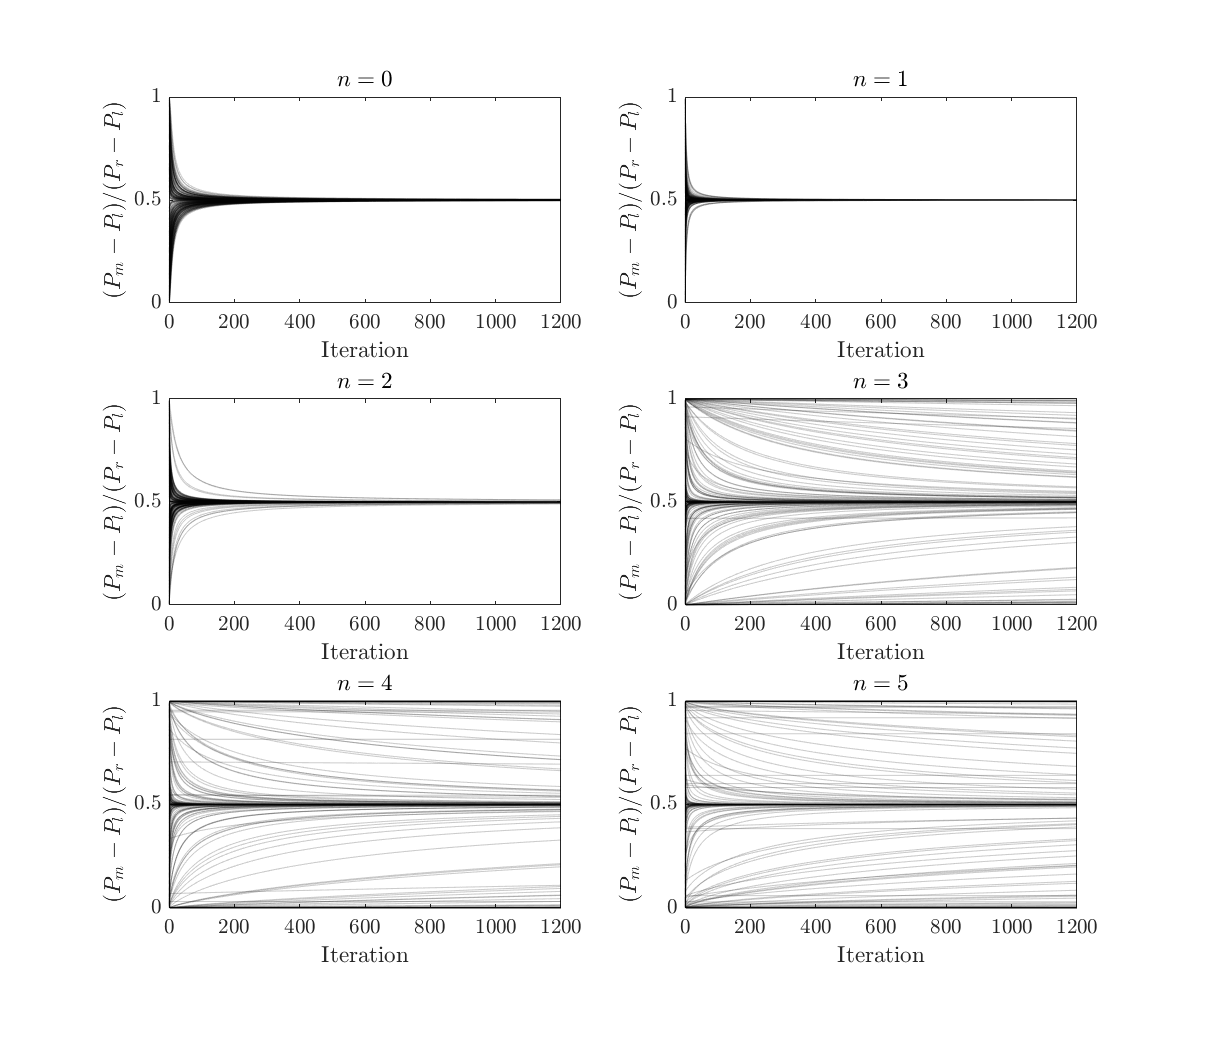
\includegraphics[width=1\textwidth]{./Figs/toy-model-series}}
\caption{Toy model for two pipes in seris. In each iteration, we
  change the radius of the pipe as $r_{\text{new}} = r_{\text{old}} +  \alpha Q/r_{\text{old}}^n$}
\label{toy-series}
\end{figure}  


\newpage
\subsection{Two Parallel Pipes Case}
%
Now assume two pipes in parallel as shown in Fig. \ref{figure:resistor-series-par}.
%
\begin{figure}[ht]
  \begin{center}
    \begin{circuitikz}
      \draw
      (-0.5,0) node[anchor=east] {$P_{l}$} to [short] (0.1,0)
      -- (0.1,0.5) 
       to[R=$1/C_1$] (2,0.5)  -- (2,0) to [short] (2.5,0) node
       [anchor=west] {$P_r$};
      \draw
      (0.1,0)  --(0.1,-0.5) 
       to[R=$1/C_2$] (2,-0.5)  -- (2,0);
    \end{circuitikz} 
    \caption{Two resistors parallel together} \label{figure:resistor-series-par}
  \end{center}
\end{figure}
%
In this case, first we have
%
\begin{align}
  Q_1 = C_1 \Delta P, \quad \text{ and }\quad Q_2 = C_2 \Delta P \\
  Q = (C_1 + C_2) \Delta P
\end{align}
%
We change the radius of each pipe according to its flow, as a result,
we have
%
\begin{align}
  \frac{dr_{1}}{dt}  = \alpha \frac{Q_{1}}{r_{1}^n}, \qquad  \frac{dr_{2}}{dt}  = \alpha \frac{Q_{2}}{r_{2}^n} \\
  r_1^n \frac{dr_{1}}{dt}  + r_2^n \frac{dr_{2}}{dt}  = \alpha (Q_1 + Q_2) = \alpha Q  
\end{align}
%
On the other hand, we know that
%
\begin{align}
  \Delta P = \frac{Q_{1}}{C_{1}}  = \frac{Q_{2}}{C_{2}} \\
  \Delta P = \frac{Q_{1}}{\beta r_1^{4}}  = \frac{Q_{2}}{\beta r_2^{4}}   \\
  \frac{dr_{i}}{dt}  = \alpha \frac{Q_{i}}{r^{n}_{i}} = \frac{\alpha \beta \Delta P}{r^{n-4}_{i}}   
\end{align}
%

We have
%
\begin{align}
  &r_{1}^{n-4} \frac{dr_{1}}{dt} = r_2^{n-4}\frac{dr_{2}}{dt}\\
  &\text{if }n=3, \quad \to \log(\frac{r_{1}}{r_{1,0}}) = \log(\frac{r_{2}}{r_{2,0}}), \to r_1 = \gamma r_2 \\
  & \text{if }n\neq 3, \quad r_1^{n-3} - r_2^{n-3} = \gamma
\end{align}
%
where $\gamma$ is a constant. In the above equation, without loss of
generality, we can assume that $r_{1}>r_2$ and $\gamma$ is
positive. Now, looking at the other part of the equation, we have
%
\begin{align}
  \frac{dr_{2}}{dt}  & = \alpha \frac{Q_2}{r^4_{2}} =  \frac{\alpha \beta \Delta P}{r^{n-4}_{2}} \\
                     & = \frac{\alpha \beta }{r^{n-4}_{2}} \frac{Q}{\beta (r_{2}^{4} + r_1^4)} = \frac{\alpha Q}{r^{n}_{2} + r_{2}^{n-4} r_1^{4}} \\
                     & = \frac{\alpha Q}{r^{n}_{2} + r_{2}^{n-4} \lp r_2^{n-3} + \gamma \rp^{\frac{4}{n-3} }}\\
  \lb r^{n}_{2} + r_{2}^{n-4} \lp r_2^{n-3} + \gamma \rp^{\frac{4}{n-3} }\rb dr_2 & = \alpha Q dt\\
  \frac{1}{n+1} \lb r_2^{n+1} + \lp r_2^{n-3} + \gamma\rp^{\frac{n+1}{n-3} }\rb  & = \alpha Qt + C\\
  r_2^{n+1} + \lp r_2^{n-3} + \gamma\rp^{\frac{n+1}{n-3} }  & = (n+1)\lp \alpha Qt + C\rp \\
  r_2^{n+1} + r_{1}^{n+1} = At+B
\end{align}
%
So the two set of equations summarizes to
%
\begin{align}
  r_1^{n-3} - r_2^{n-3} &= \gamma \\
  r_1^{n+1} + r_2^{n+1} &= At + B
\end{align}
%
The plot for the solution to the above equations for different values
of $n\neq 3$ and also the separate solution for $n=3$ is shown in the
following figure.  
%

\begin{figure}[h]
  \centerline{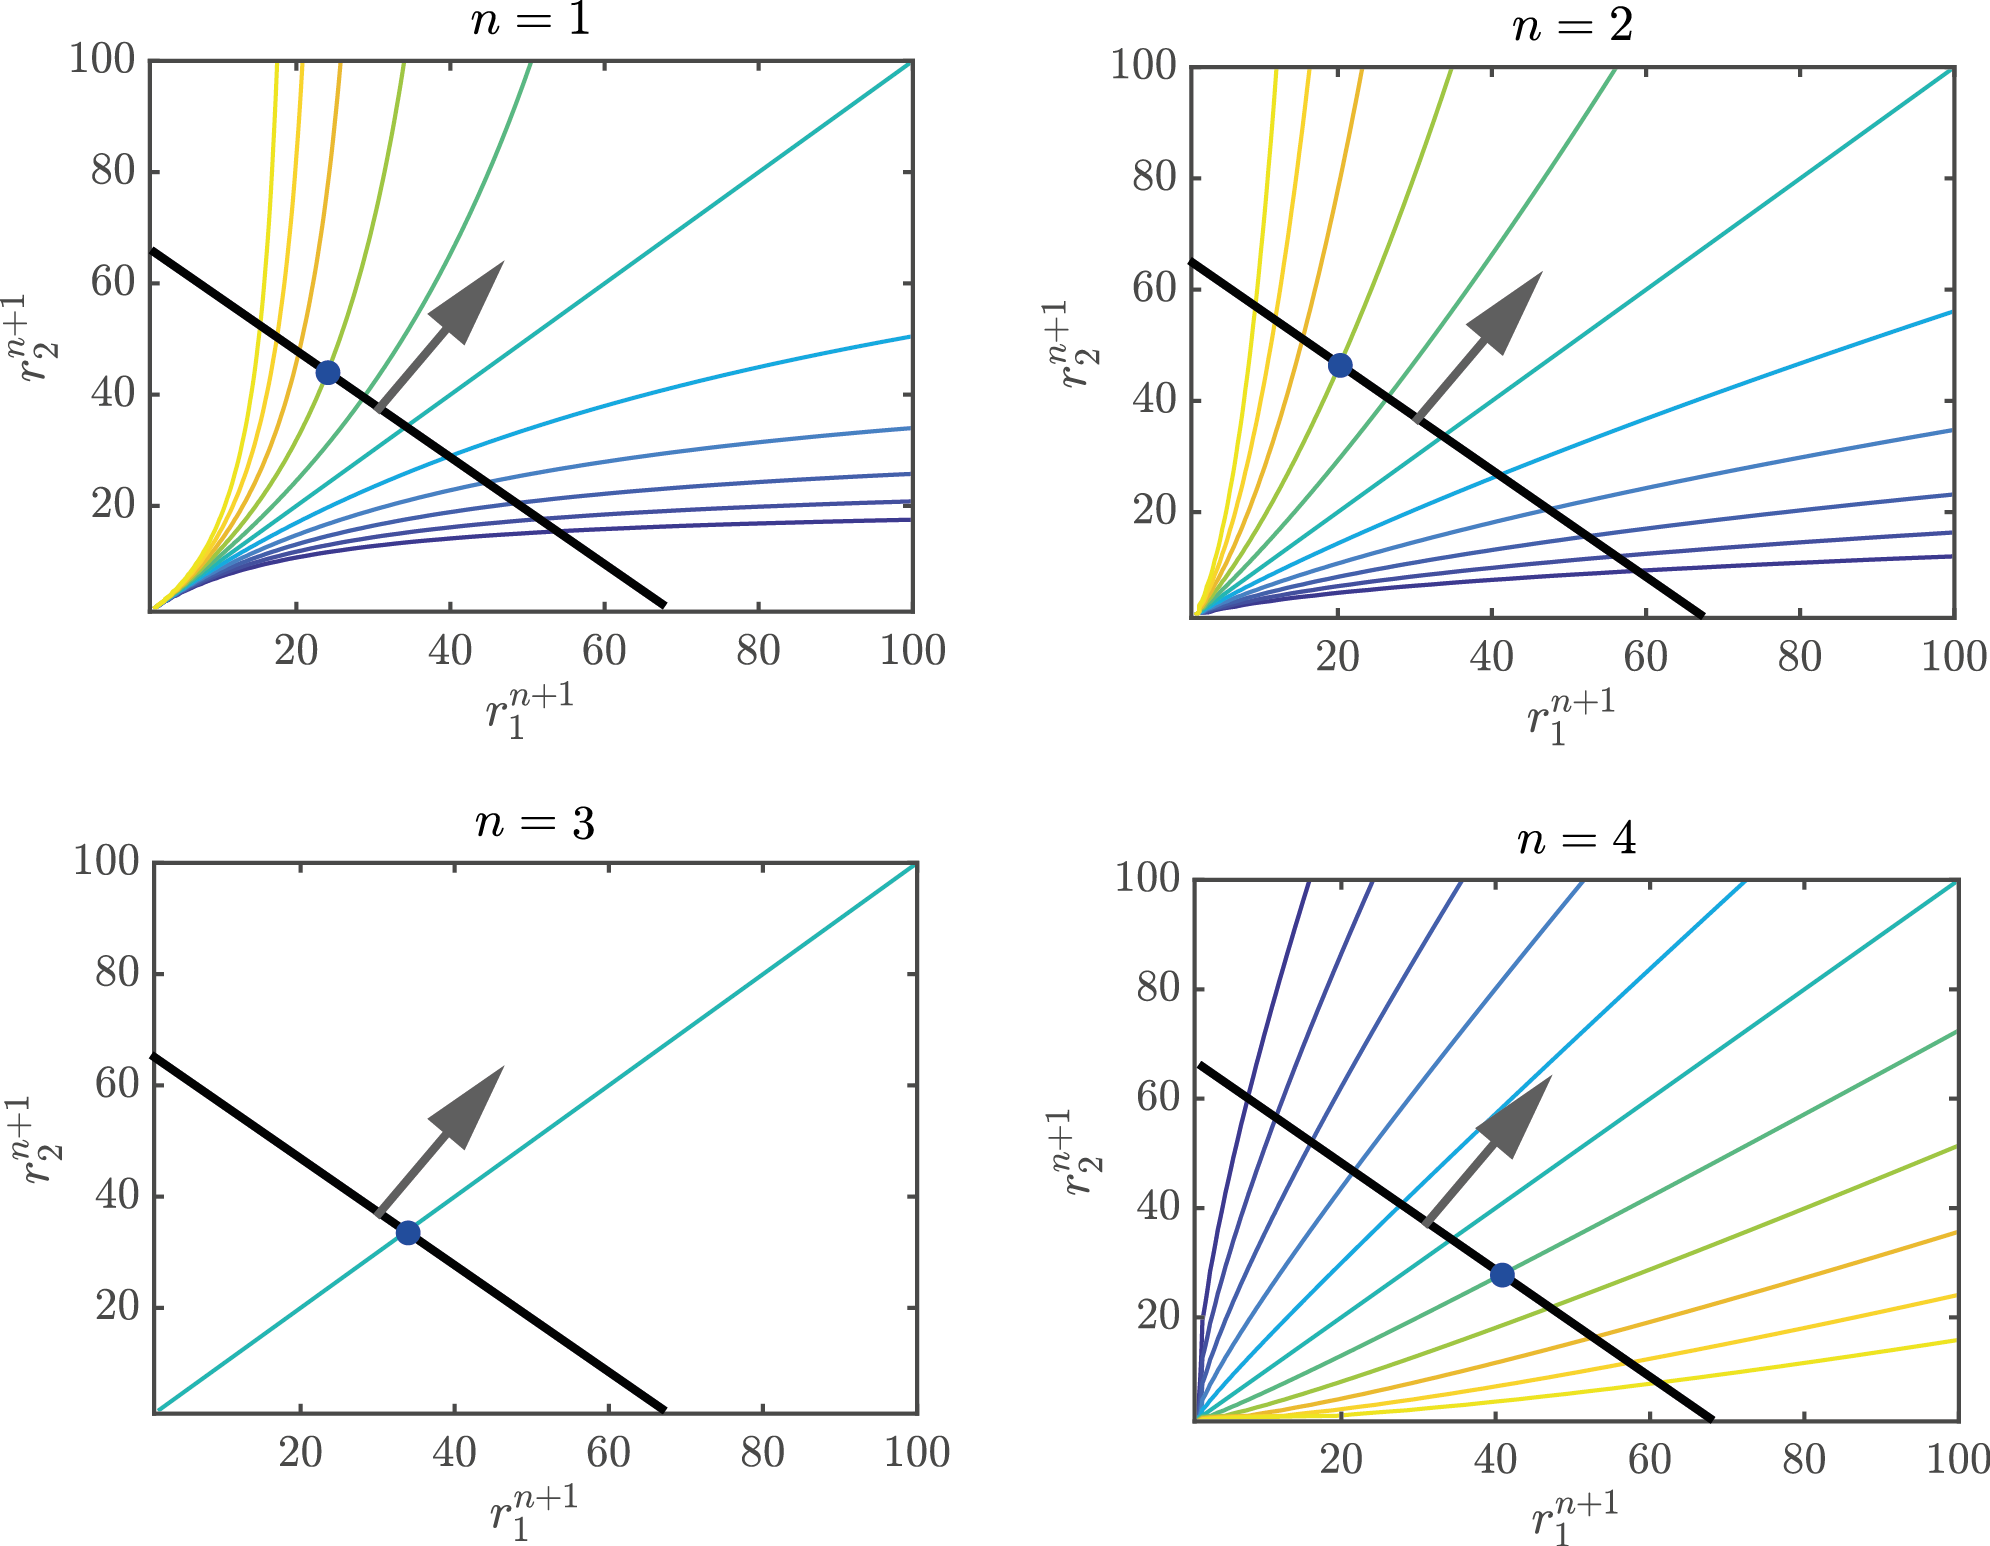
\includegraphics[width=0.8\textwidth]{./Figs/par_resistors}}
  \caption{Analytical solution for $r_1$ and $r_2$ for parallel
    resistors. For different $n$ the solution changes. Specifically,
    if $n<3$, then one of the diameters stops varying while the other
    one increases in size. If $n=3$, the both grow together, and if
    $n>3$ then they both increase in size. }
\label{anal-par}
\end{figure}  


The result for numerical simulation is shown in Fig. \ref{toy-par}.


\begin{figure}[h]
  \centerline{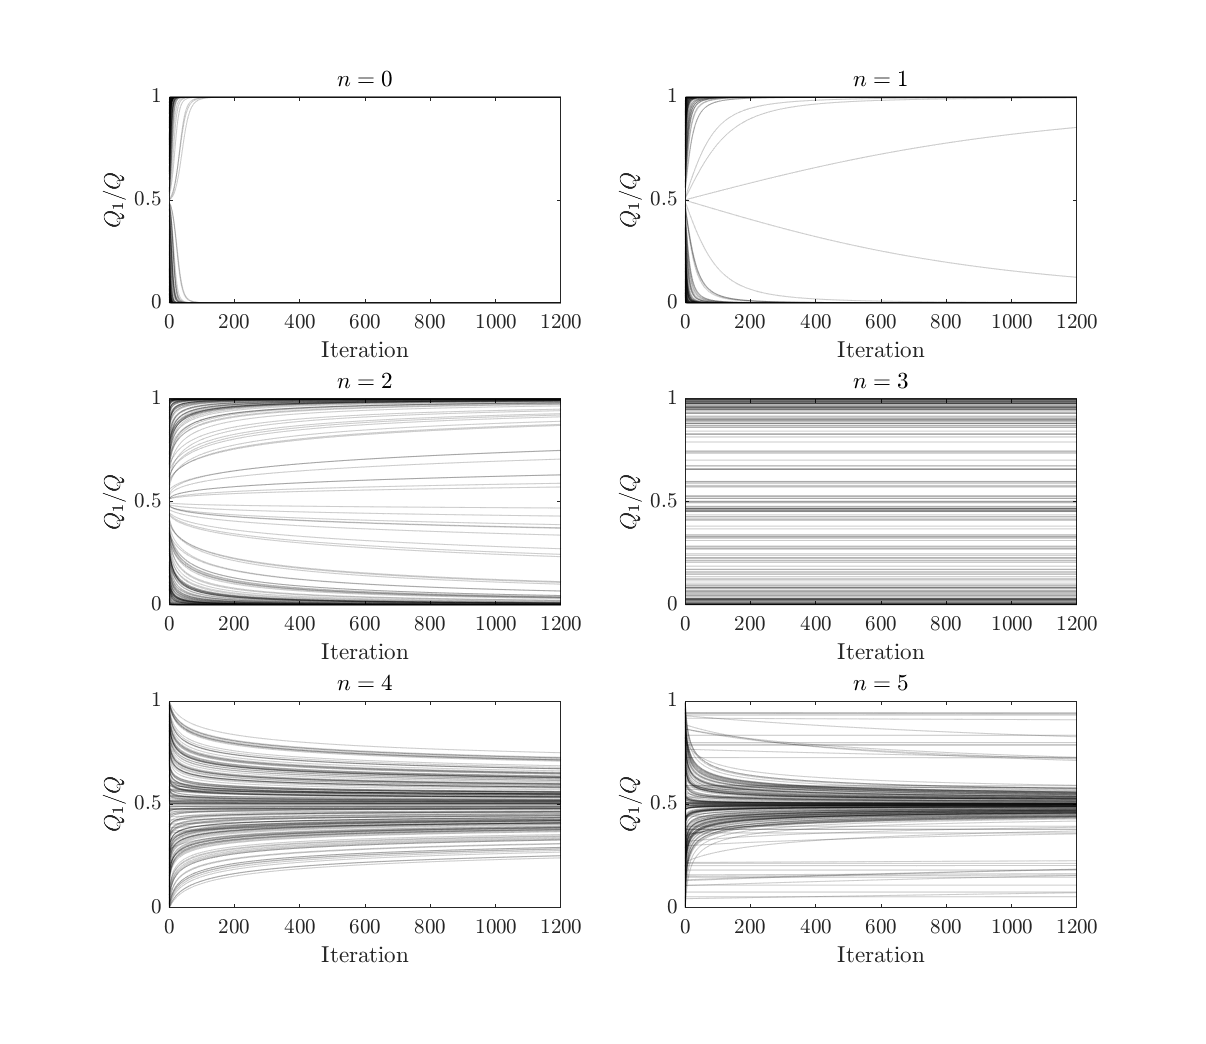
\includegraphics[width=1\textwidth]{./Figs/toy-model-par}}
\caption{Toy model for two pipes in parallel. In each iteration, we
  change the radius of the pipe as $r_{\text{new}} = r_{\text{old}} +  \alpha Q_{i}/r_{\text{old}}^n$}
\label{toy-par}
\end{figure}  

Another way of seeing this and also generalize the results is to study the change of relative radius $\tilde{r}_1 = \frac{r_1}{r_1+r_2}$ under the assumptions 
\begin{equation}
    C_i = r_i^m, ~ \frac{dr_i}{dt}= \alpha \frac{Q_i}{r_i^n}.
\end{equation}
It can be easily derived that 
\begin{equation}
    \frac{d\tilde{r_1}}{dt} \propto \tilde{r}_1 (1-\tilde{r}_1) \frac{r_1^{m-n-1}-r_2^{m-n-1}}{r_1^m+r_2^m},
\end{equation}
which has  a fixed point at either 1.  $\tilde{r_1} = 0$ or $1$ or 2.$r_1=r_2$. The first case is the channeling and the second case is the uniform. It can also be shown that if $m-n-1>0$ the system ends at channelling, otherwise uniform except when $m-n-1=0$ it will end up with no change of the relative radius.

\newpage

\subsection{Parallel and Series}
%
Now, we assume a combination of both parallel and series case as shown
in Fig. \ref{resistor-par-series}. The top and bottom series part,
become more and more homogeneous for any flow that passes through
them. However, the flow between top and bottom separates based on the
power of $n$.
%
\begin{figure}[ht]
  \begin{center}
    \begin{circuitikz}
      \draw
      (-0.5,0) node[anchor=east] {$P_{l}$} to [short] (0.1,0)
      -- (0.1,0.5) 
       to[R=$1/C_1$] (2,0.5) to[R=$1/C_2$] (4,0.5) -- (4,0) to [short] (4.5,0) node
       [anchor=west] {$P_r$};
      \draw
      (0.1,0)  --(0.1,-0.5) 
       to[R=$1/C_3$] (2,-0.5) to[R=$1/C_{4}$] (4,-0.4)--(4,0);
    \end{circuitikz} 
    \caption{Parallel/Series Case} \label{resistor-par-series}
  \end{center}
\end{figure}

\subsubsection{Corrections (Deng)}
Numerical simulations show different result here for more complex cases other than naive parallel or series cases. For example for the following case Fig \ref{resistor-par-series21}.
\begin{figure}[ht]
    \begin{center}
    \begin{circuitikz}
      \draw
      (-0.5,0) node[anchor=east] {$P_{l}$} to [short] (0.1,0)
      -- (0.1,0.5) 
       to[R=$1/C_1$] (2,0.5)  --  (4,0.5)  -- (4,0) to [short] (4.5,0) node
       [anchor=west] {$P_r$};
      \draw
      (0.1,0)  --(0.1,-0.5) 
       to[R=$1/C_2$] (2,-0.5) to[R=$1/C_{3}$] (4,-0.4)--(4,0);
    \end{circuitikz} 
    \caption{Parallel/Series Case (Deng)} \label{resistor-par-series21}
  \end{center}
\end{figure}
The simulations are similar to previous ones that keep the flow constant while increasing the radius proportional to $Q/r^n $. It now shows that the flow does not need to be homogeneous through top and bottom tubes. A special case can be easily analytically calculated. Set $C_{1}(t=0) = 2, C_{2}(t=0)=C_{3}(t=0) = 1$, and let $n=7$, in this case 
\begin{equation}
    \frac{dC_i}{dt} = 4Q_i/C_i
\end{equation}
and $C_2=C_3$ will always hold, and it is not difficult to solve $C_1$ and $C_2$
\begin{align}
    \frac{dC_1}{dt} = \frac{8Q}{C_2+2C_1} \\
    \frac{dC_2}{dt} = \frac{4Q}{C_2+2C_1},
\end{align}
where $Q$ is the total flow. In fact we do not need to solve these simple equations and it is clear that at the end we get $C_2=C_3=1/2 C_1$ since $\frac{dC_1}{dC_2} = 2$. However, this means at the end $Q_1/Q = 4/5$ instead of $1/2$. 



\newpage
\section{Toy Model - Clogging}
%%
\begin{align}
  \frac{d r}{dt} & = - \alpha \frac{Q}{r^{n}} 
\end{align}
%
\subsection{Series - Numerical result}
%
We assume the following pattern for the resistors \ref{figure:resistor-series-clogging}
%
\begin{figure}[h]
  \begin{center}
    \begin{circuitikz}\draw
      (0,0) node[anchor=east] {$P_{l}$} to [short,o-] (0.1,0)
       to[R=$1/C_{1}$,-*] (2,0)  node [anchor=north] {$P_m$}
       to[R=$1/C_2$] (4,0)
       to[short,-o] (4.1,0) node [anchor=west] {$P_r$}; % The resistor
    \end{circuitikz}
    \caption{Two resistors at series}\label{figure:resistor-series-clogging}
  \end{center}
\end{figure}
%
The numerical simulation results are shown in
Fig. \ref{toy-series-clog}.
%
\begin{figure}[h]
  \centerline{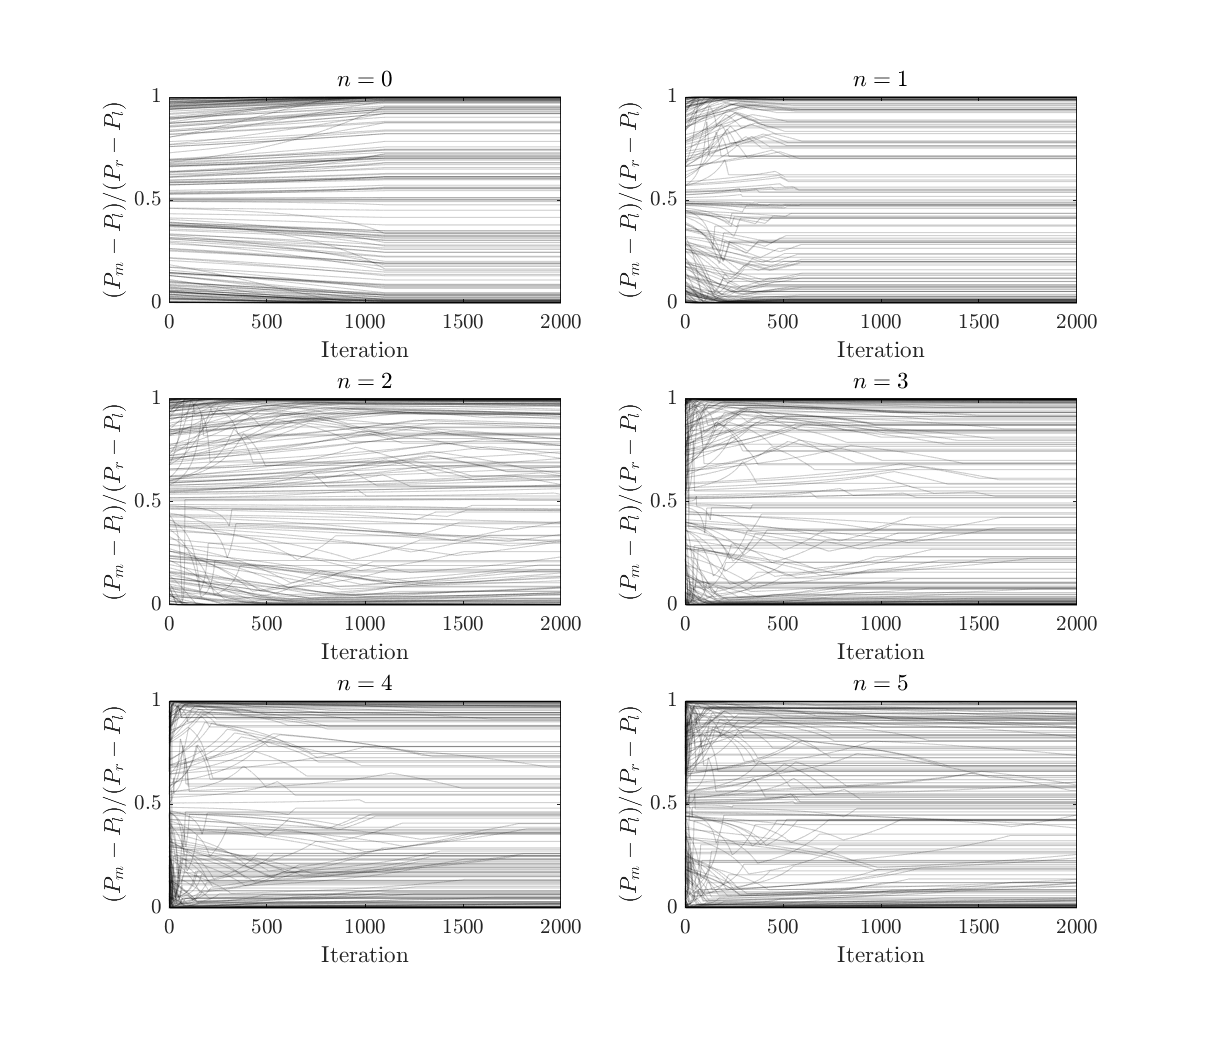
\includegraphics[width=1\textwidth]{./Figs/toy-model-series-clog}}
  \caption{Toy model for two pipes in series. In each iteration, we
    change the radius of the pipe as
    $r_{\text{new}} = r_{\text{old}} - \alpha
    Q_{i}/r_{\text{old}}^n$. Note that we set a maximum change of
    $\Delta r = \min{1,r}$.}
\label{toy-series-clog}
\end{figure}  


\subsection{Parallel - Numerical result}
%
We assume the following pattern for the resistors \ref{figure:resistor-par-clogging}
%
\begin{figure}[ht]
  \begin{center}
    \begin{circuitikz}
      \draw
      (-0.5,0) node[anchor=east] {$P_{l}$} to [short] (0.1,0)
      -- (0.1,0.5) 
       to[R=$1/C_1$] (2,0.5)  -- (2,0) to [short] (2.5,0) node
       [anchor=west] {$P_r$};
      \draw
      (0.1,0)  --(0.1,-0.5) 
       to[R=$1/C_2$] (2,-0.5)  -- (2,0);
    \end{circuitikz} 
    \caption{Two resistors parallel together} \label{figure:resistor-par-clogging}
  \end{center}
\end{figure}





The numerical simulation results are shown in
Fig. \ref{toy-par-clog}.
%
\begin{figure}[h]
  \centerline{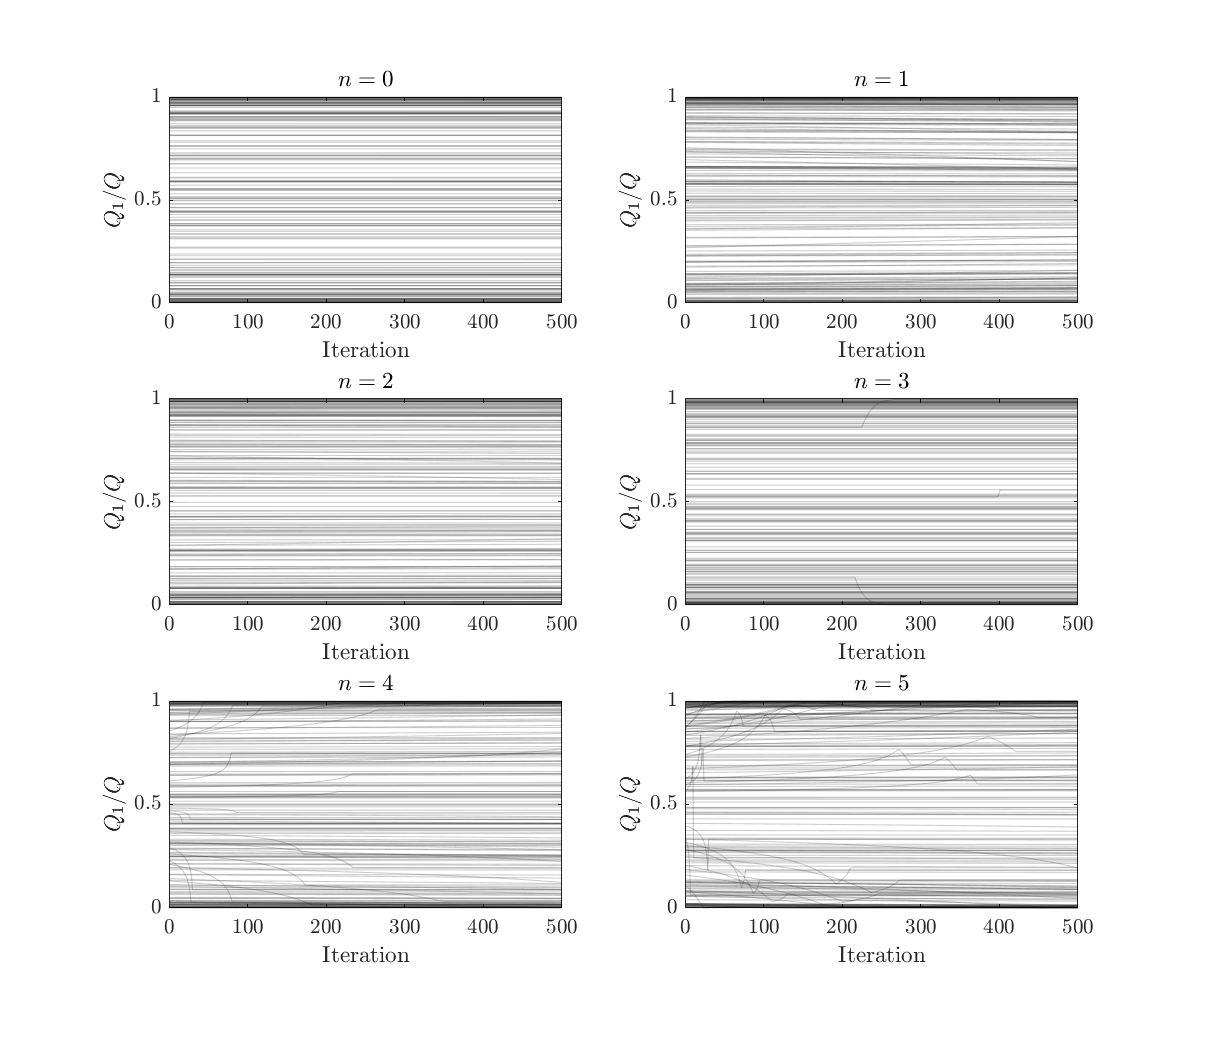
\includegraphics[width=1\textwidth]{./Figs/toy-model-par-clog}}
  \caption{Toy model for two pipes in series. In each iteration, we
    change the radius of the pipe as
    $r_{\text{new}} = r_{\text{old}} - \alpha
    Q_{i}/r_{\text{old}}^n$. Note that we set a maximum change of
    $\Delta r = \min{1,r}$.}
\label{toy-par-clog}
\end{figure}  







\newpage

\section{Localization Degree}
%
In channelling, sparsity of flow occurs. In other words, most of the
flow passes through few pipes. The measures already used to calculate
sparsity are the following
%

\begin{center}
  \begin{tabular}{ |c|l|l| }
    \hline
  Measure & Definition & Description  \\ \hline
    $\ell^{0}_{\ep}$  & $\#\{j, q_j \leq \ep \}$ & \\ \hline
    $-\ell^p$ & $-\lp \sum_j q_j\rp^{1/p}$ & \\ \hline
    $\ell^2/\ell^1$ & $\sqrt{\sum_j q_j^2}/\sum_j q_j$ &\\ \hline
    $\kappa_4$ & $\sum_j q_j^4 / \lp \sum_{j} q^{2}_{j}\rp^2$ & \\ \hline
    $-\log$ & $-\sum_j \log \lp 1 + q_j^2\rp $ & \\ \hline
    $-\tanh_{a,b}$ & $-\sum_j \tanh \lp a q_j^b\rp$ & \\
\hline                               
\end{tabular}
\end{center}


The following measures I propose based on our problem
%
\begin{align}
  \mathcal{L}_1 = \frac{1}{N - 1} \lp N - \frac{\lp \sum_{j} q_j\rp ^2}{\sum_jq^2_j} \rp\\
  \mathcal{L}_2 = \frac{1}{N - 1} \lp N - \frac{\lp \sum_{j} q_j^{2}\rp^2}{{\sum_jq^4_j}} \rp    
\end{align}
%
In the above measures if $q$ is uniform and the same everywhere, then
the measure is $\mathcal{L}_1 = \mathcal{L_2} = 0$. The extreme
heterogeneity case the measure goes toward $1$. The resulting videos
are Movie S1 and S2. 

\section{Generalization of conductance erosion law (Deng)}
Here is a naive guess of how the exponent of erosion law can change the network topology. We can assume the erosion law  
\begin{align}
    C &= a r^m \\
    \frac{dr}{dt} &= \frac{b Q}{r^n},
\end{align}
where $a,b,m,n$ are some constants. It can be derived that it is equivalent to
\begin{equation}
    \frac{dC}{dt} \propto QC^{1-\frac{n+1}{m}}.
\end{equation}
Particularly in previous series/parallel cases, $m=4$ and $n$ varies. We observed that $n<3$ leads to channeling while $n>3$ leads to homogeneity. Therefore, a reasonable guess is with the erosion law 
\begin{equation}
    \frac{dC}{dt} \propto Q^\alpha C^\beta,
\end{equation}
when $\alpha = 1$, the sign of $\beta$ will determine the channeling behavior. And the simulations as shown in Fig. \ref{fig:erosionExp} confirm the guess. Furthermore, we can see the change of flow distribution in terms of $P(Q)$, the distribution of flow in every resistor, as shown in Fig \ref{fig:PQ}. The exponential tail remains in the simulations for the $\beta = 0$ case.
\begin{figure}[h]
  \centerline{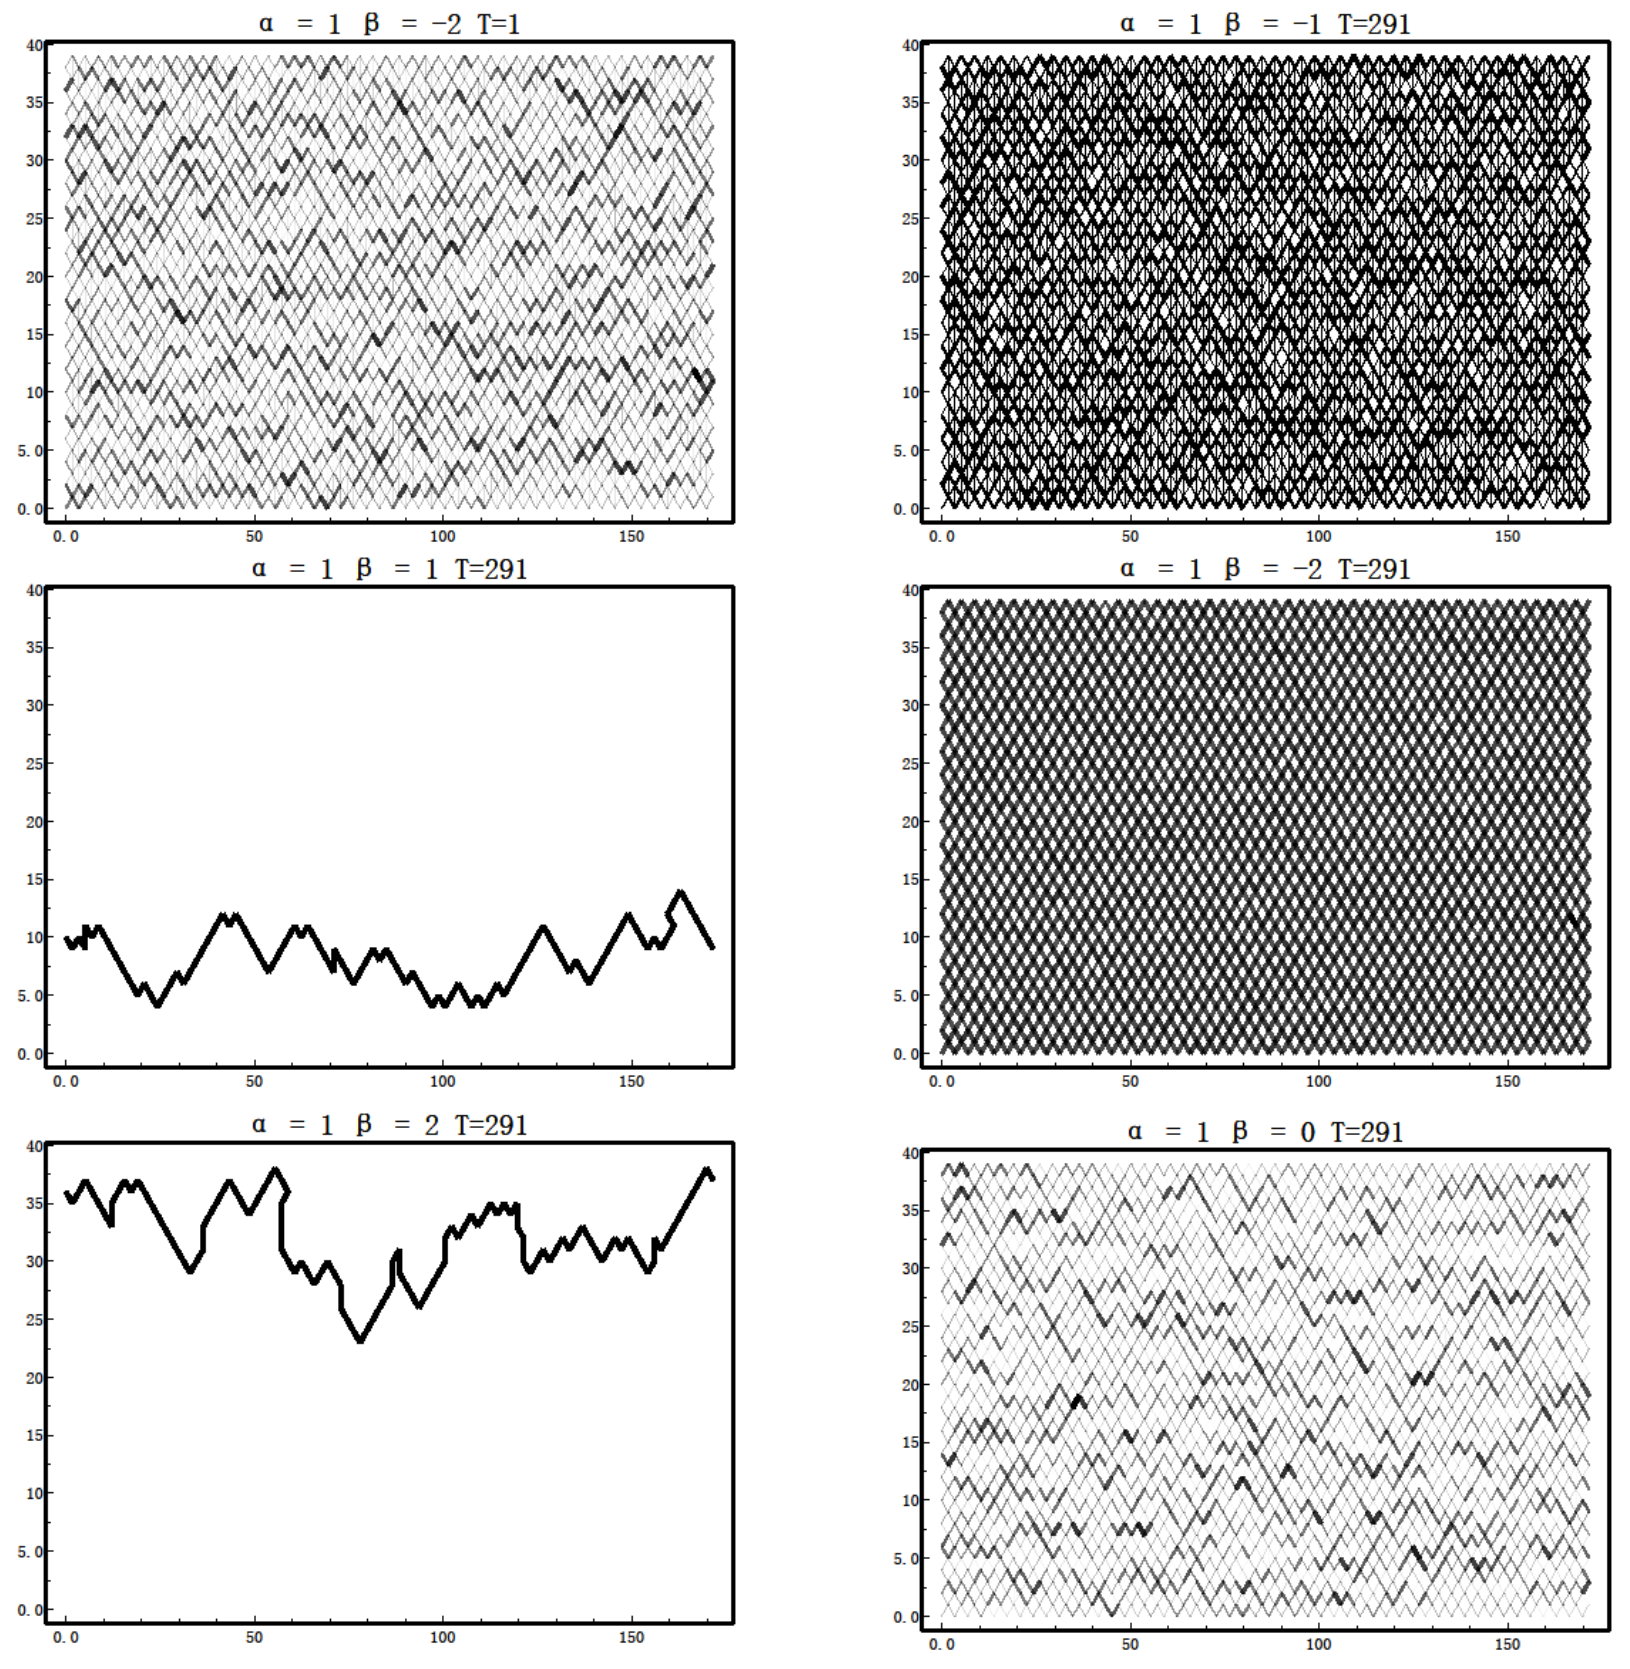
\includegraphics[width=1\textwidth]{./Figs/erosionExp.png}}
  \caption{A grid network erosion simulations with different $\beta$ exponents. Top left is the initial flow distribution for every simulation (T=1) and the rest are final distributions of the flow.}
\label{fig:erosionExp}
\end{figure}  

\begin{figure}
    \centering
    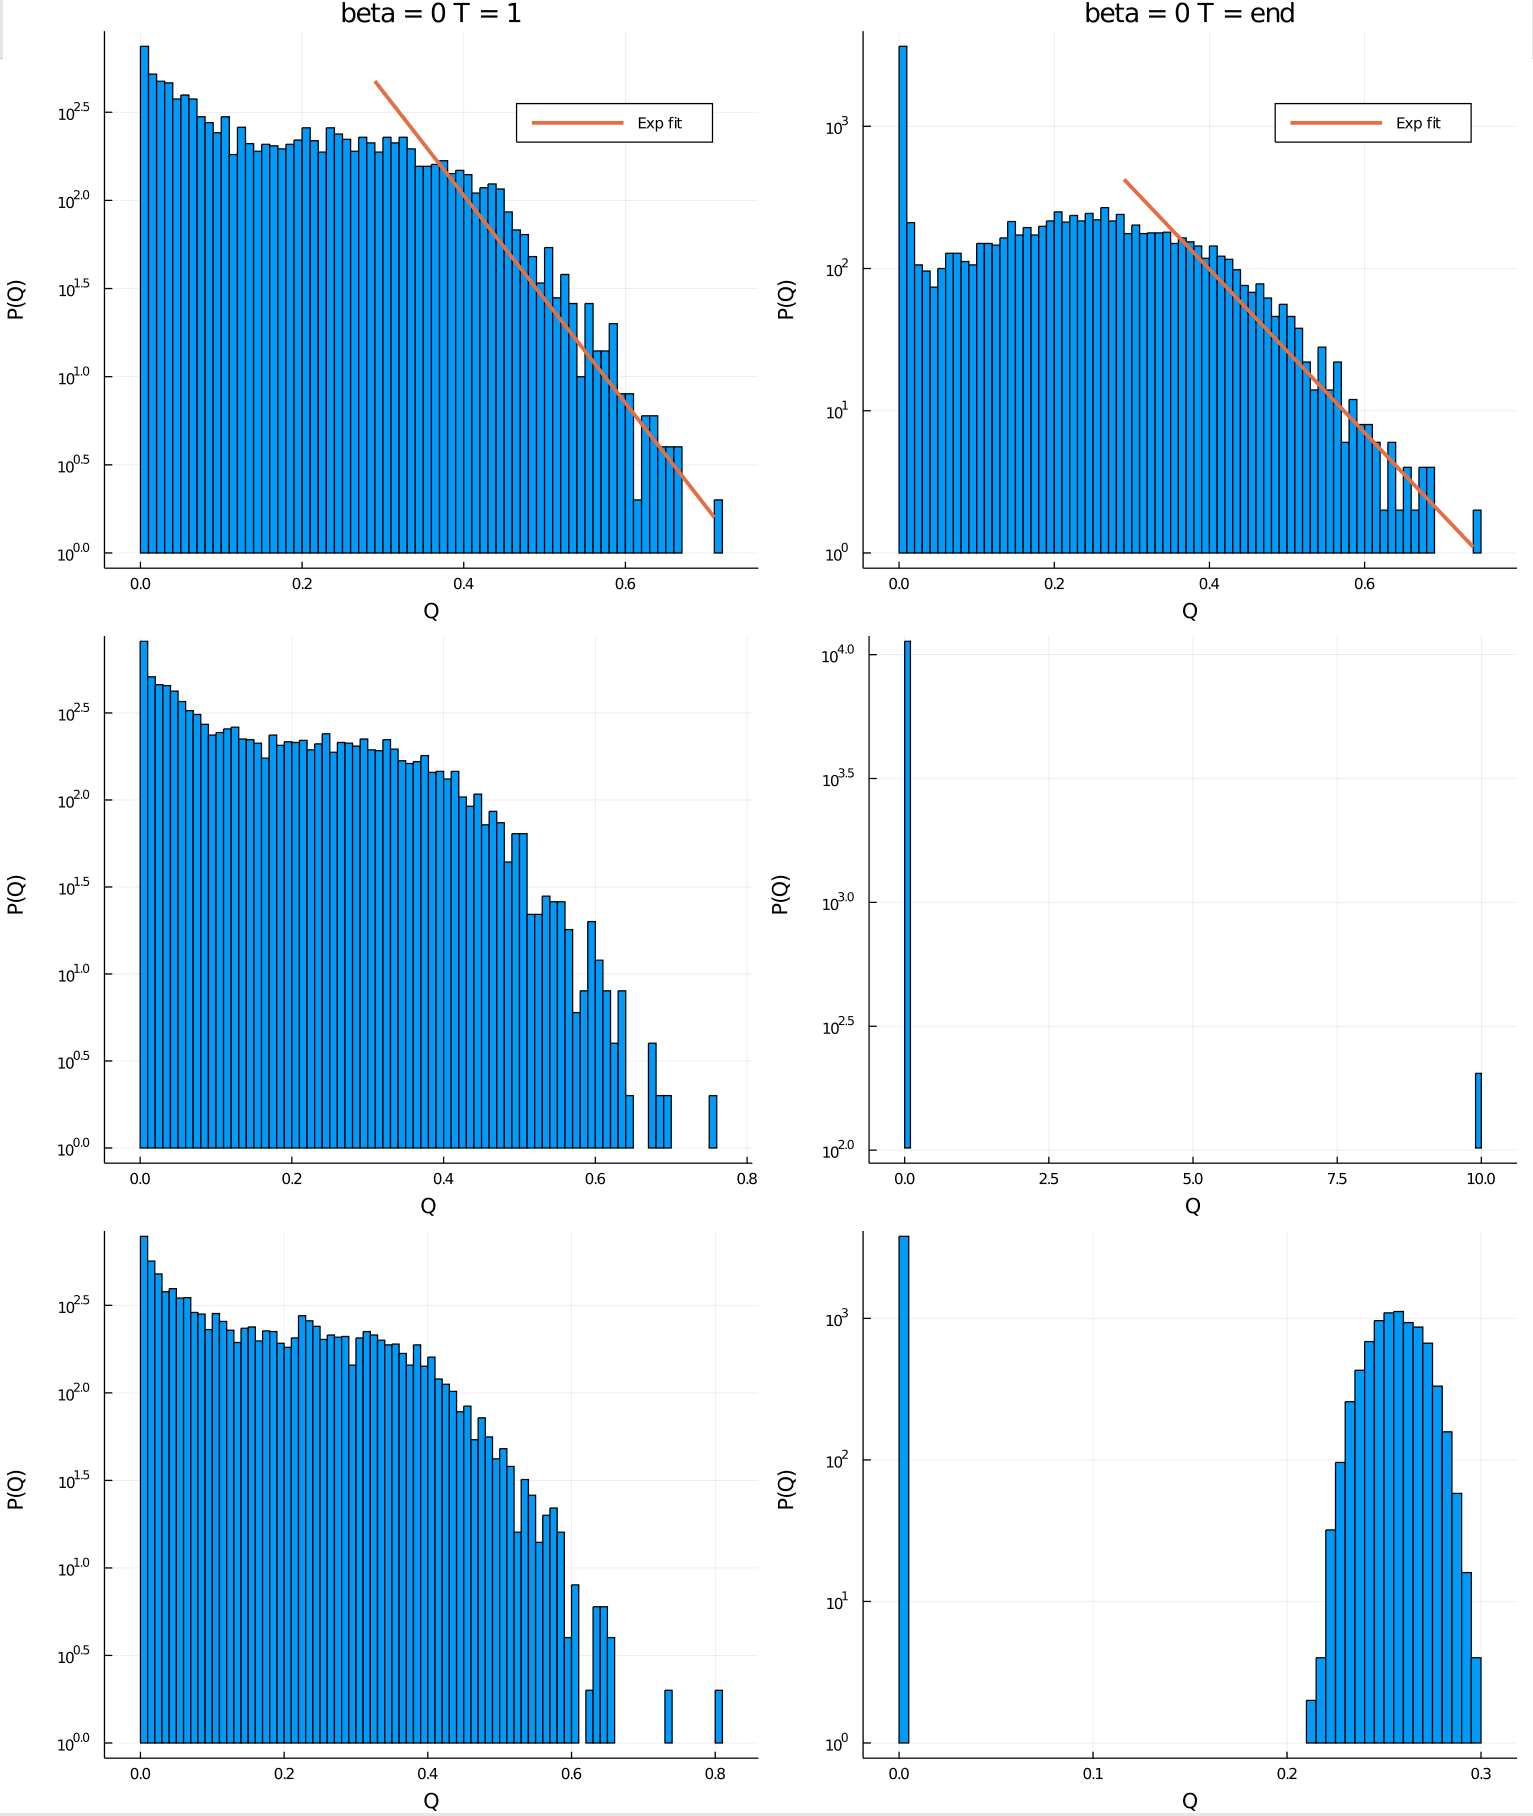
\includegraphics[width = 0.8\textwidth]{Figs/PQ.png}
    \caption{The flow distribution of networks in Fig \ref{fig:erosionExp} for different $\beta$'s. It is easy to distinguish channeling ($\beta = 1$), homogeneity ($\beta = -1$) and exponential tail ($\beta = 0$) from the flow distributions at the end of simulations.  }
    \label{fig:PQ}
\end{figure}


\bibliography{ref}


\end{document}



\section{Shear Rate Homogenity}
%
In the numerical simulation, we observe that after changing the radius
of the pipes with the following dynamics 
%
\begin{align}
  \frac{d r}{dt } = \alpha \frac{Q}{r^{3}} 
\end{align}
%
the flow becomes more homogeneous, i.e. the pressure versus the
position becomes almost linear.

\section{Two Pipe Study}
%
Let's consider two pipes connected as shown blow
%
\begin{figure}[h]
 \centerline{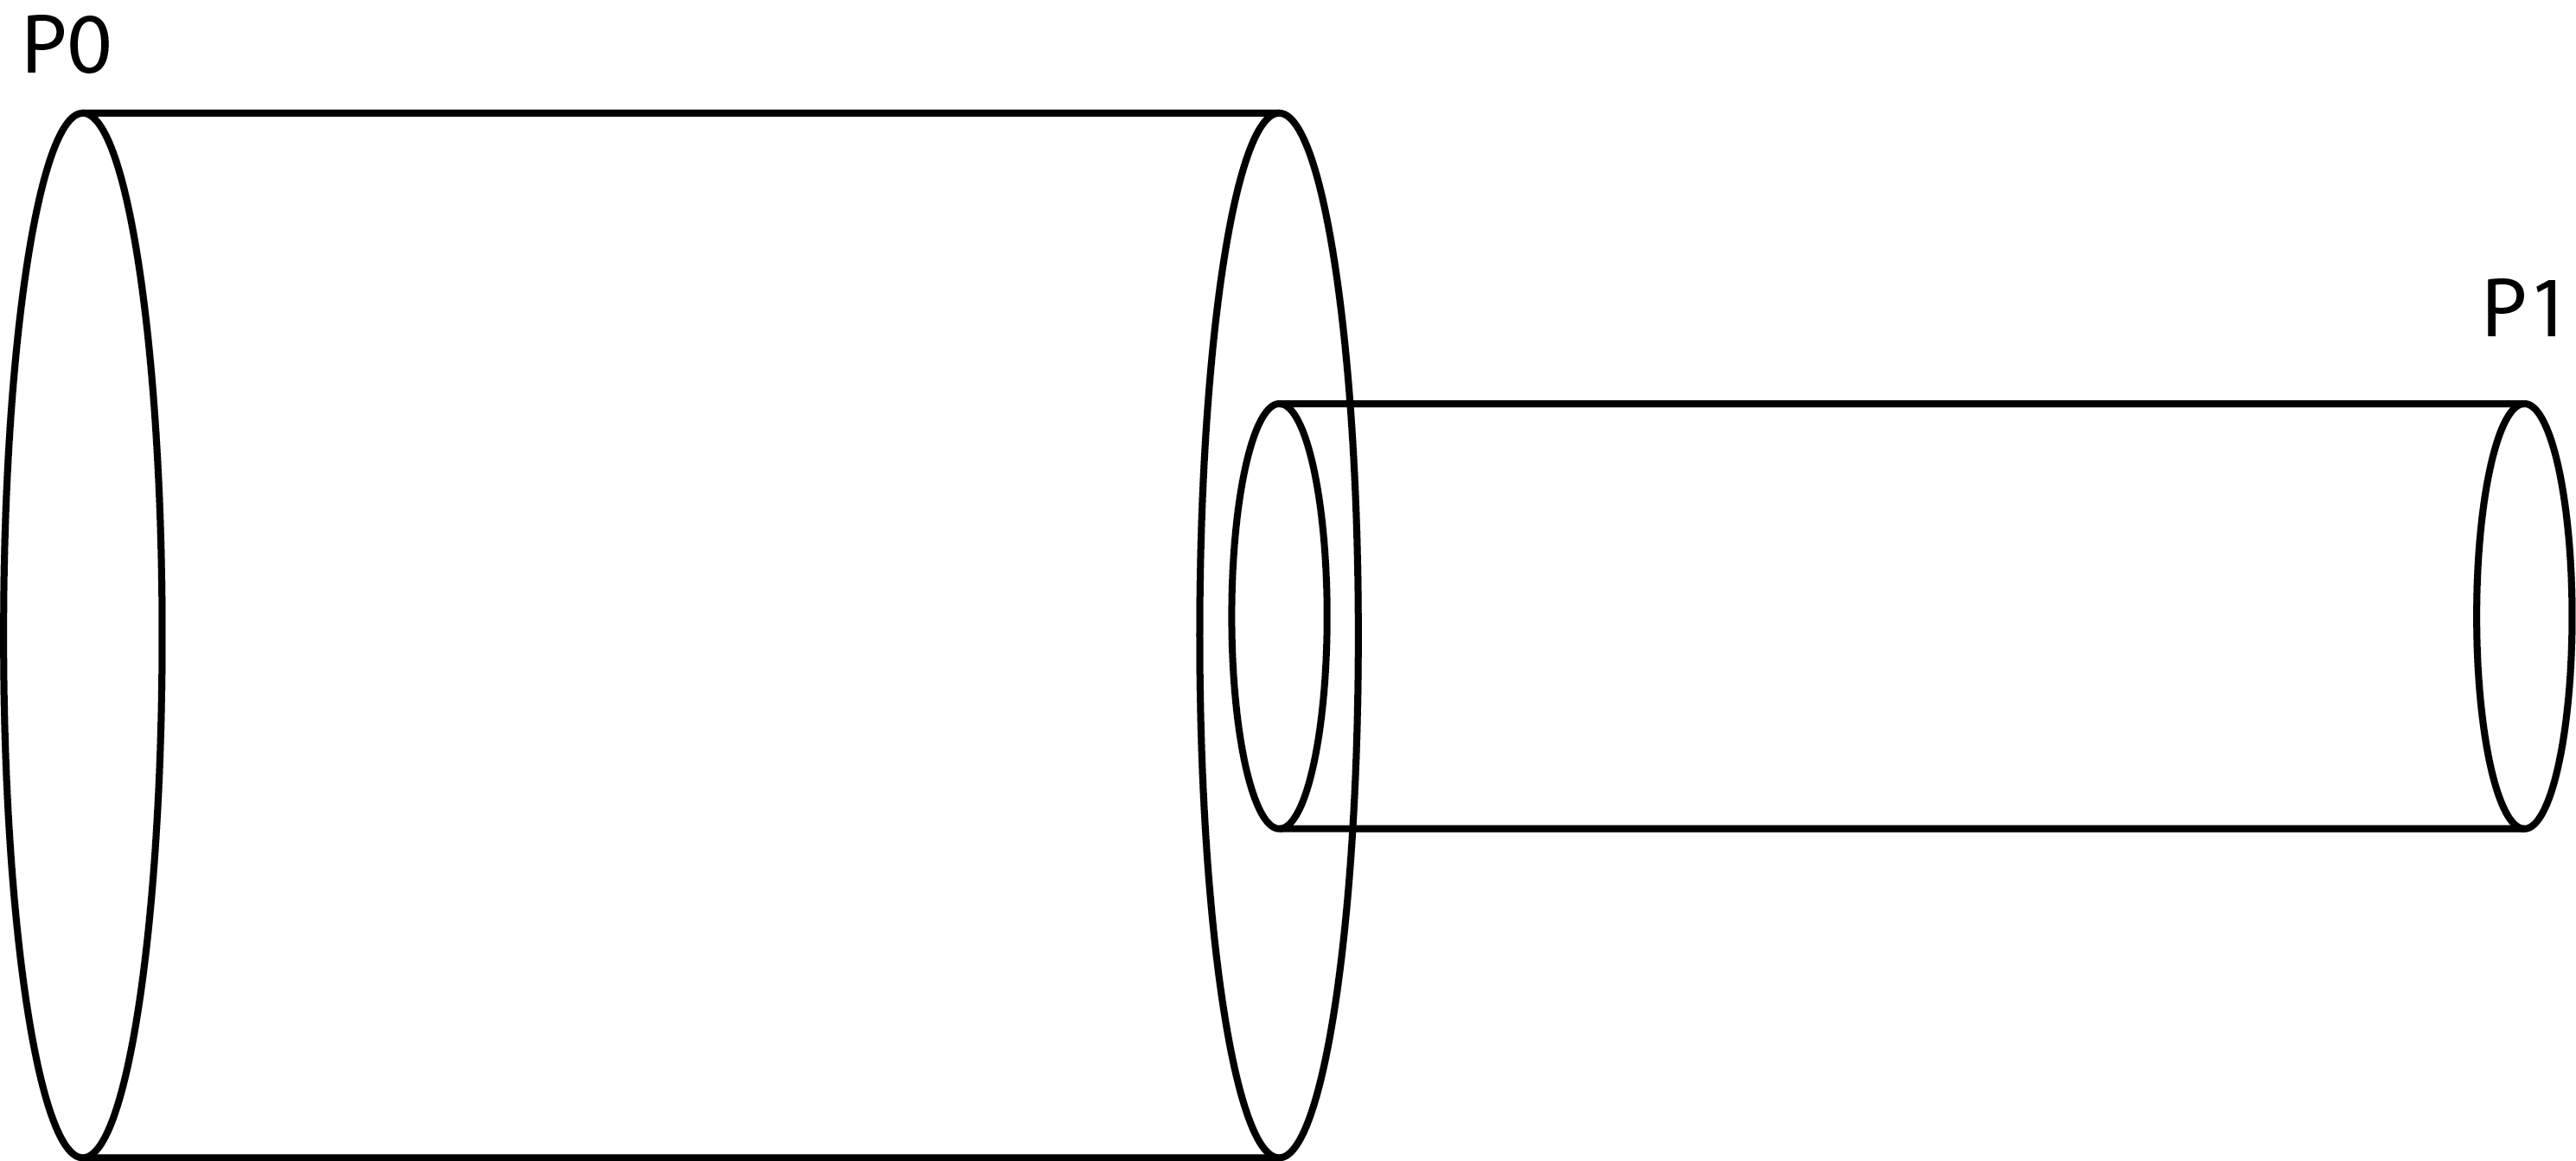
\includegraphics[width=.4\textwidth]{./Figs/twopipes}}
\caption{Two pipe model}
\label{sup-fig4}
\end{figure}  
%
We assume $P_0$ on one side and $P_1$ on the other side. The flow $Q$
and pressure difference are related as follows
%
\begin{align}
  &Q = -\frac{\pi r^4}{8\mu L} {\Delta P} \\
  &\boxed{Q = \sigma (r) \Delta P, \quad \sigma(r) =   -\frac{\pi r^4}{8\mu L}}\\
  & R(r) Q = \Delta P, \quad R(r) =  -\frac{8\mu L}{\pi r^4}
\end{align}
%
For the two pipe system we have
%
\begin{align}
  Q & = \sigma(r_1) (P_m - P_0) \\
  Q & = \sigma (r_2) (P_1- P_m) \\
  & \to \quad Q \lp \frac{1}{\sigma(r_{1})} + \frac{1}{\sigma(r_{2})}  \rp = P_1 - P_0
\end{align}
%
Solving for pressure at the middle point we have $P_m $
%
\begin{align}
  P_m = P_0 + \frac{{1}/{\sigma(r_{1})} }{{1 }/{\sigma(r_{1})} + {1}/{\sigma(r_{2})} } (P_1 - P_0) \\
  \boxed{P_m = P_0 + \frac{\sigma(r_2)}{\sigma(r_1) + \sigma(r_2)} (P_1 - P_0)}
\end{align}
%
Note that for the dynamics we know that
%
\begin{align}
  & \boxed{\frac{d r}{dt } = \alpha \frac{Q}{r^{3}}}  \\
  & r^3 \frac{d r}{d t}   = \alpha Q \\
  & \frac{d}{dt} r^4 = \alpha Q  \\ 
  & \boxed{\frac{d}{dt} \sigma(r) = \alpha \frac{\pi}{8\mu L} Q = \text{const.}}
\end{align}
%

\begin{figure}[h]
 \centerline{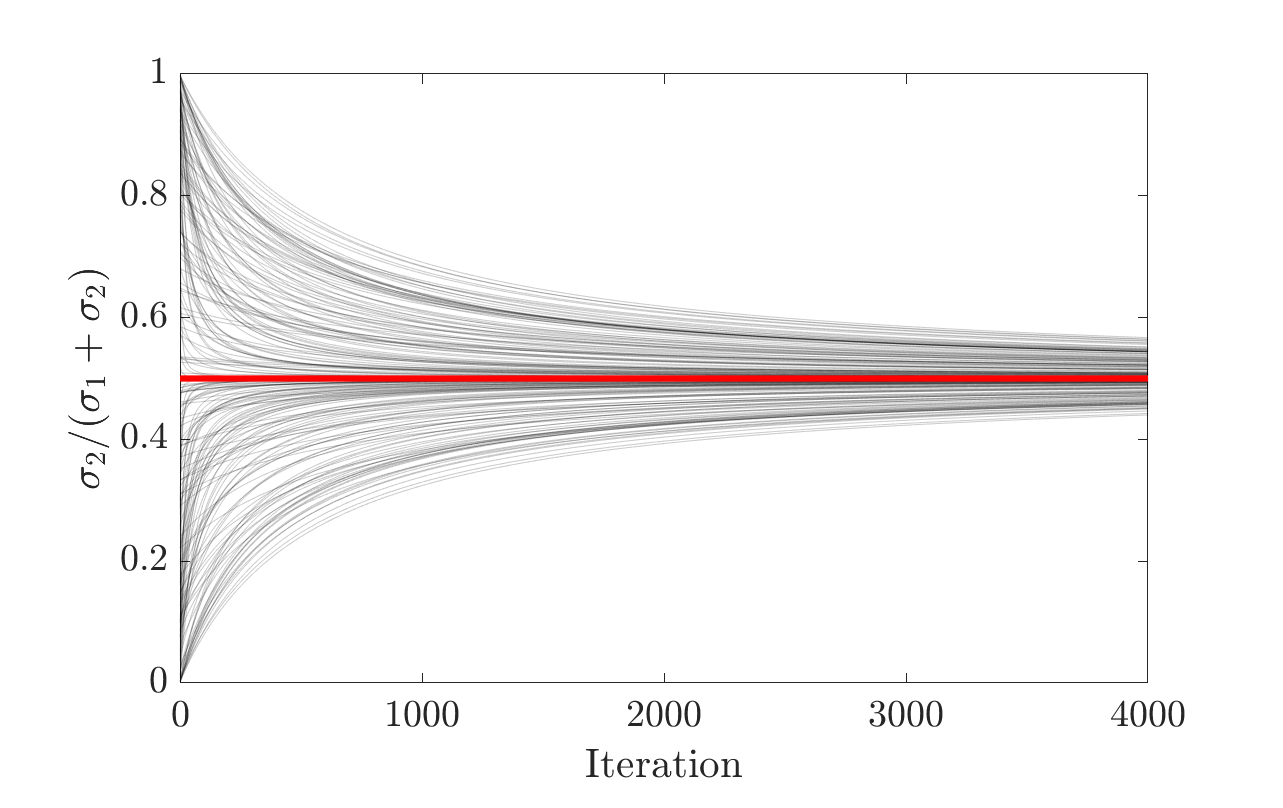
\includegraphics[width=.75\textwidth]{./Figs/shear-iterations}}
\caption{Increasing conductivity at a constant rate}
\label{sup-fig4}
\end{figure}  



\subsection{General dependence}
%
Lets assume a general dynamics equation as
%
\begin{align}
  & \frac{dr}{dt}  = \alpha \frac{Q}{r^{n}} \\
  & r^3 \frac{d r}{d t}   = \alpha \frac{Q}{r^{n-3}}  \\
  & \frac{d}{dt} r^4 = \alpha \frac{Q}{r^{n-3}} \\ 
  & \boxed{\frac{d}{dt} \sigma(r) \propto \frac{Q}{\sigma^{(n-3)/4}}   }
\end{align}
%
In the following I have the results for different N
%
% \begin{figure}[h]
%   \centerline{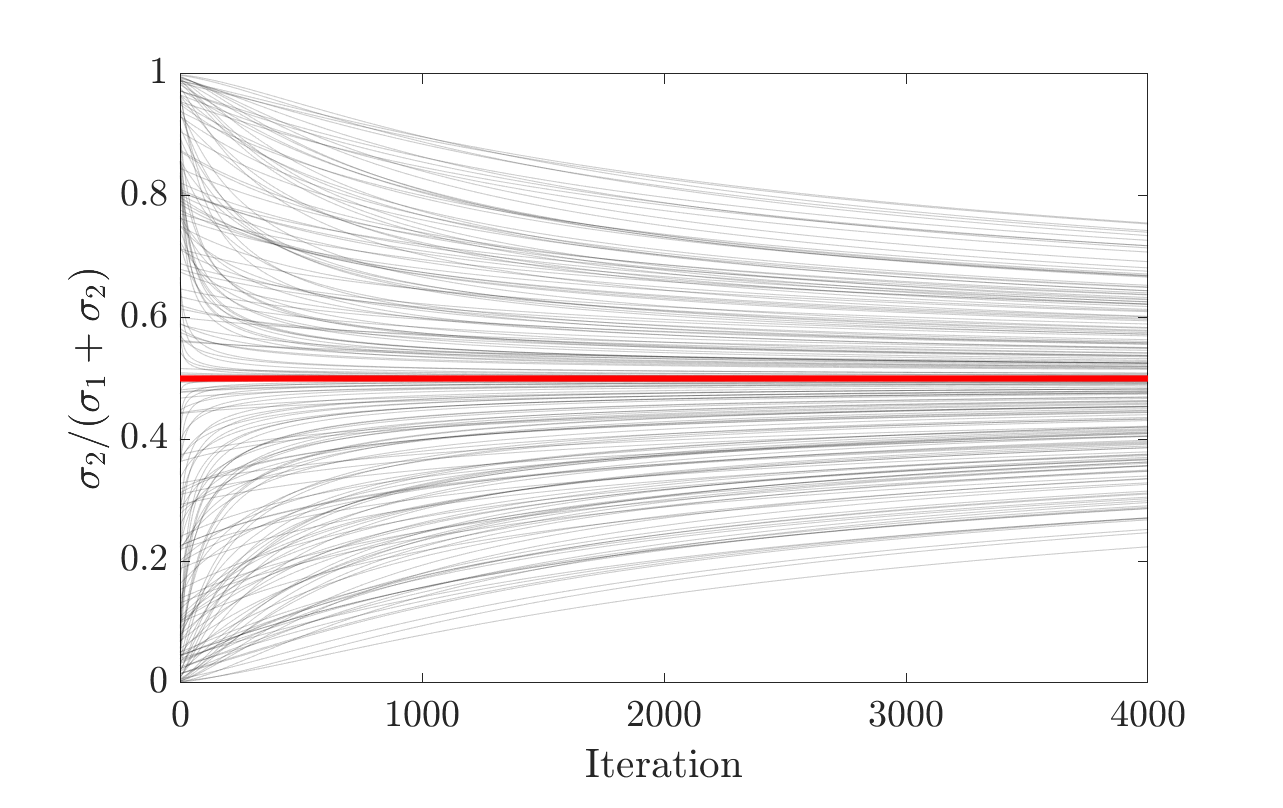
\includegraphics[width=.5\textwidth]{./Figs/shear-iterations_n1}}
%   \centerline{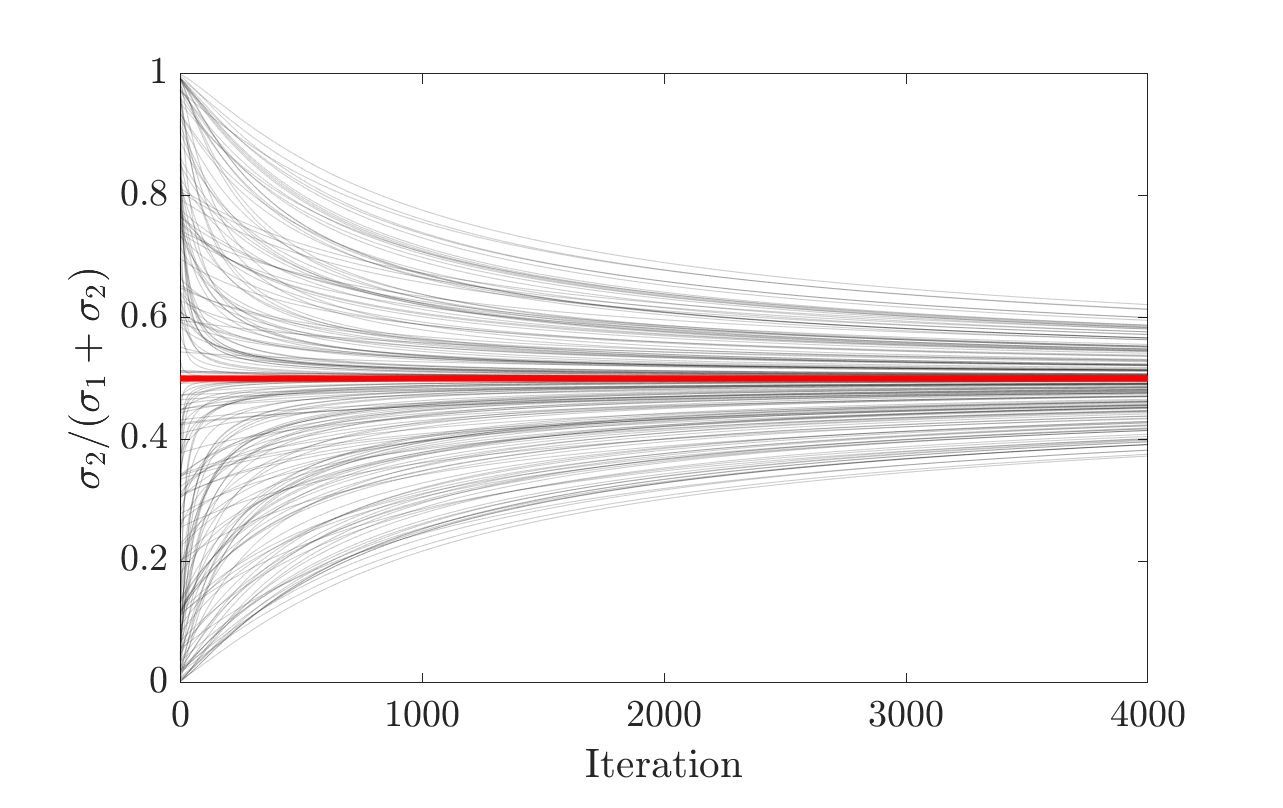
\includegraphics[width=.5\textwidth]{./Figs/shear-iterations_n2}}
%   \centerline{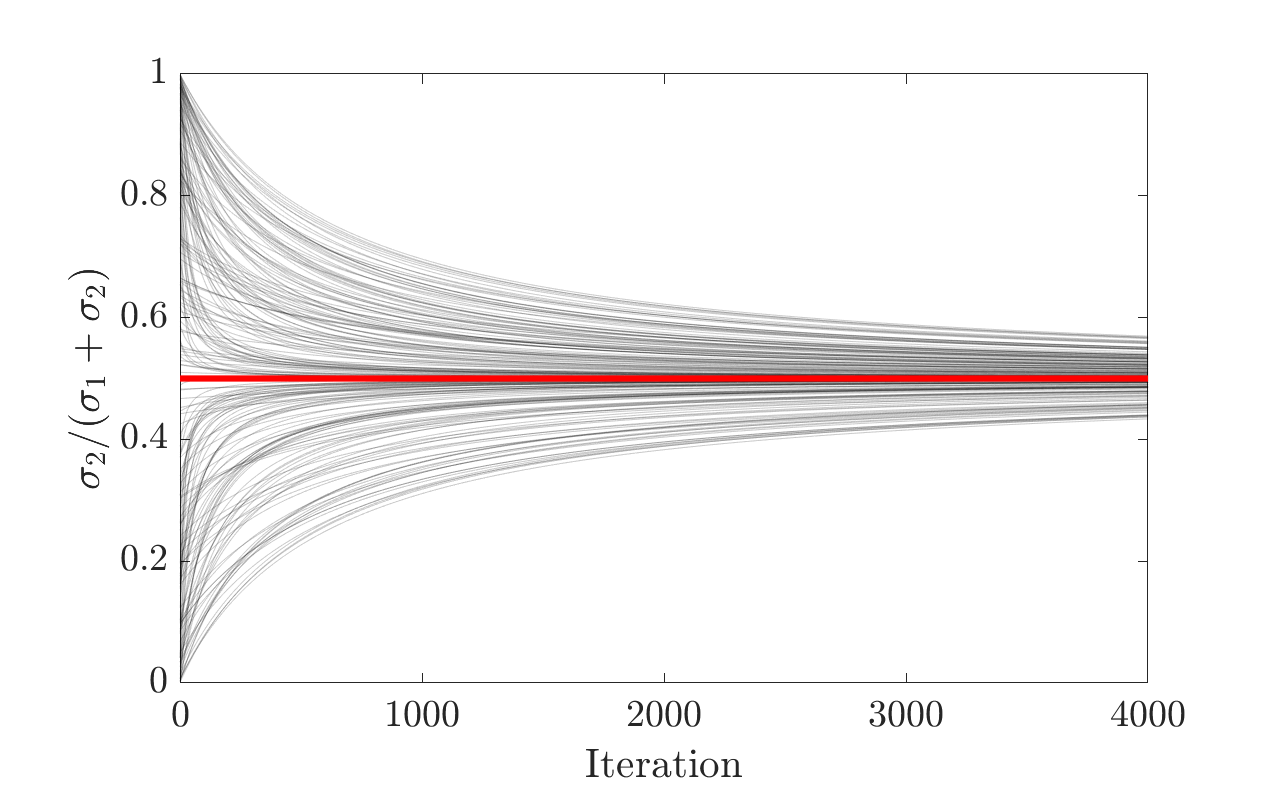
\includegraphics[width=.5\textwidth]{./Figs/shear-iterations_n3}}
%   \centerline{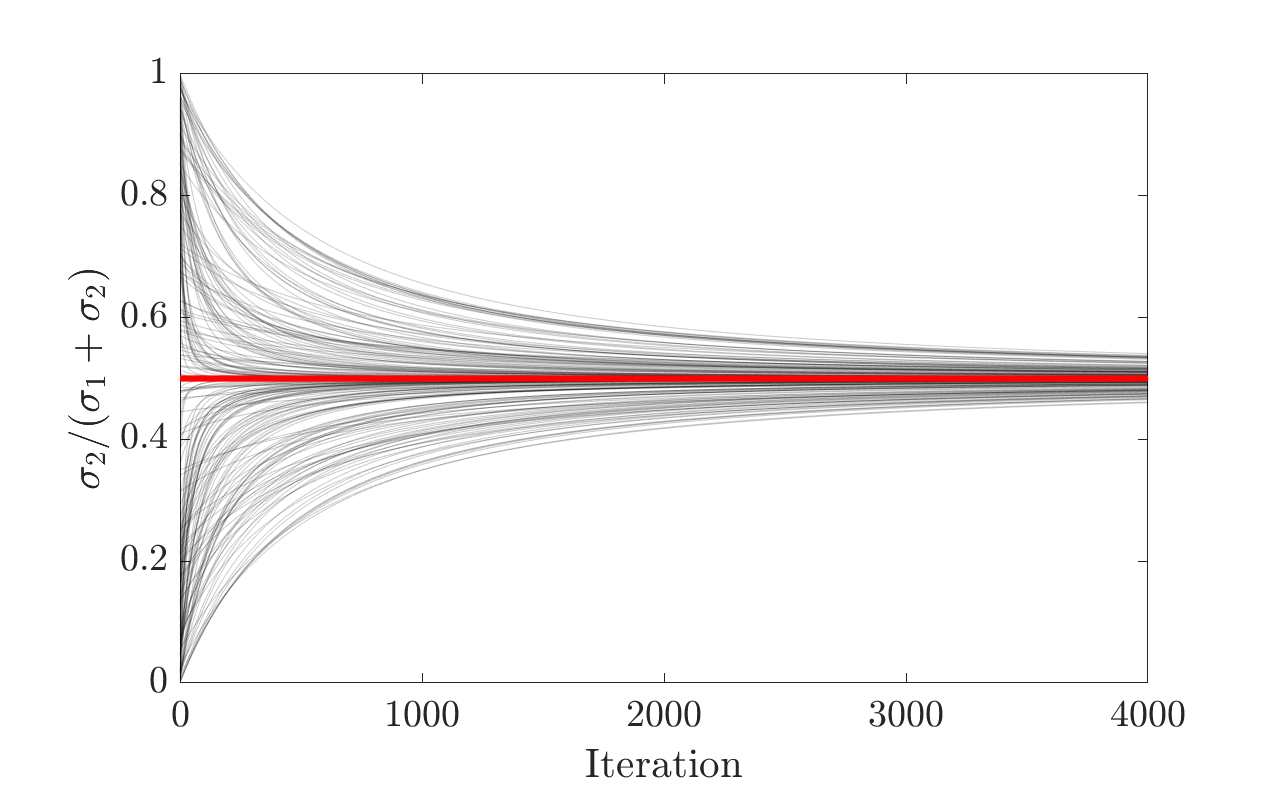
\includegraphics[width=.5\textwidth]{./Figs/shear-iterations_n4}}
% \caption{Increasing conductivity at a constant rate}
% \label{sup-fig4}
% \end{figure}  




\subsection{Three in Series}
%
Now assume three pipes back to back as shown in Fig. \ref{figure:resistor-series-2}.
%
\begin{figure}[h]
  \begin{center}
    \begin{circuitikz}\draw
      (0,0) node[anchor=east] {$P_{l}$} to [short,o-] (0.1,0)
       to[R=$1/C_1$,-*] (2,0)  node [anchor=north] {$P_m$}
       to[R=$1/C_2$] (4,0) to[R=$1/C_3$] (6,0) 
       to[short,-o] (6.1,0) node [anchor=west] {$P_r$}; % The resistor
    \end{circuitikz}
    \caption{Three resistors at series}
  \end{center}\label{figure:resistor-series-2}
\end{figure}
%
\begin{align}
  Q &= \frac{1}{1/C_{1} + 1/C_2 + C_3}   \Delta P = \text{const.}, \\
  P_m - P_l &= \frac{Q}{C_{1}}   \\
  P_r - P_l &= \frac{Q}{1/C_{1} + 1/C_2 + 1/C_3}    \\
  \frac{P_{m}-P_l}{P_r - P_l} & = \frac{1/C_{1}}{1/C_{1} + 1/C_2 + 1/C_3}  
\end{align}
%
